\section{Aufbau und Durchführung}

Zu Beginn wird die Leerlaufspannung einer Monozelle gemessen. Wichtig ist es, den Eingangswiderstand $R_\text{V}$ des Voltmeters zu beachten und zu notieren. 
Nun wird die Klemmenspannung $U_\text{K}$ in Abhängigkeit des Belastungsstroms $I$ gemessen. Der Belastungswiderstand kann dabei zwischen 0-50 $\Omega$ liegen. Dazu muss die Schaltung, die in Abb. \ref{fig:2} zu sehen ist, verwendet werden.
\begin{figure}[h]
  \centering
  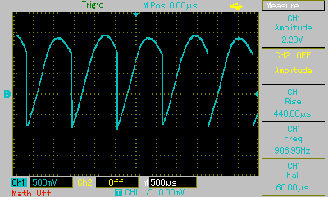
\includegraphics[height=4cm]{Grafiken/2.pdf}
  \caption{Schaltung zur Messung der Klemmenspannung $U_\text{k}$. \cite{1}}
  \label{fig:2}
\end{figure}
Als nächstes wird, wie in Abbildung \ref{fig:3} zu sehen ist, eine Gegenspannung an die Monozelle angelegt und wieder $U_\text{k}$ in Abhängigkeit von $I$ gemessen. Die Gegenspannungspannung ist dabei ungefähr 2 V größer als $U_0$. 
\begin{figure}[h]
  \centering
  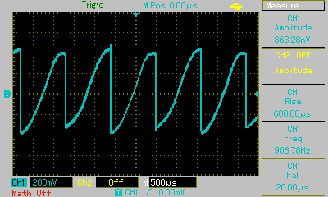
\includegraphics[height=4cm]{Grafiken/3.pdf}
  \caption{Schaltung wie Abb. \ref{fig:2}, aber mit Gegenspannung. \cite{1}}
  \label{fig:3}
\end{figure}
Im letzten Versuchsteil wird dieselbe Messung von $U_\text{k}$ vorgenommen, jedoch unter Verwendung des Sinus- und Rechteck-ausgangs eines RC-Generators anstatt der Monozelle.
Der Variationsbereich von $R_\text{a}$ des 1 V-Rechteckausgangs liegt dabei zwischen 20 - 250 $\Omega$ und der des 1 V-Sinusausgangs zwischen 0,1 - 5 k$\Omega$.
